% setup
\documentclass[hyperref={colorlinks=true},professionalfonts]{beamer}
% \usepackage[latin1]{inputenc}
\usepackage{listings}
\usepackage{hyperref}
\usepackage{graphicx}

% any shorthands
\newcommand{\us}[1]{ \_#1\_ } % we do so many underscored identifiers
\newcommand{\email}[1]{\href{mailto:#1}{#1}}

% presentation configuration
\usetheme{Dresden}
\usecolortheme{beaver}

\institute{Linux Systems Administrator \\ Rackspace, The Open Cloud Company}
\author{Martin B. Smith \\ @martinb3}

\date{\today}



\title[]{OpenStack \& The Cloud}

% document
\begin{document}

\frame{\titlepage}

\begin{frame}
The views expressed in this article are those of the author and do not necessarily represent the views of, and should not be attributed to, Rackspace.
\href{https://github.com/rackspace/social\_media\_guidelines}{Social Media Guidelines. Open Source!}
\end{frame}

\begin{frame}
\frametitle{Goals}

Goals for this presentation:
\begin{itemize}
\item Who is OpenStack?
\item What is OpenStack?
\item How can you OpenStack? \\ \medskip
\begin{center} 
\includegraphics[width=108pt]{images/sign-posts-contact-info.jpg} \end{center}
\end{itemize}

\end{frame}

\begin{frame}
\begin{center}

\includegraphics{images/openstack-cloud-software-vertical-cmyk.eps}
\end{center}
\end{frame}

\begin{frame}
\frametitle{Reply hazy, try again.}

What is the cloud?

% On-demand self-service allows users to obtain, configure and deploy cloud services themselves using cloud service catalogues, without requiring the assistance of IT.[49][50] This feature is listed by the National Institute of Standards and Technology (NIST) as a characteristic of cloud computing.

% On-demand self-service, broad network access, resource pooling, rapid elasticity, measured service

% Mention difference between capex and opex. Analogy with utilities.

% It's the internet... for compute!

\end{frame}

\begin{frame}
\begin{center}
     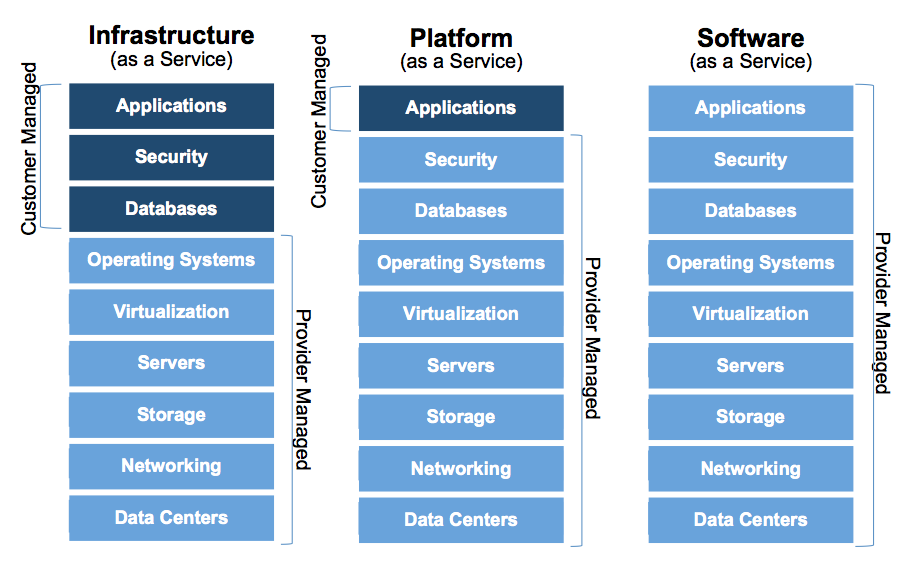
\includegraphics[width=\textwidth]{images/aas.png}
\end{center}
\end{frame}


\begin{frame}
\begin{center}
     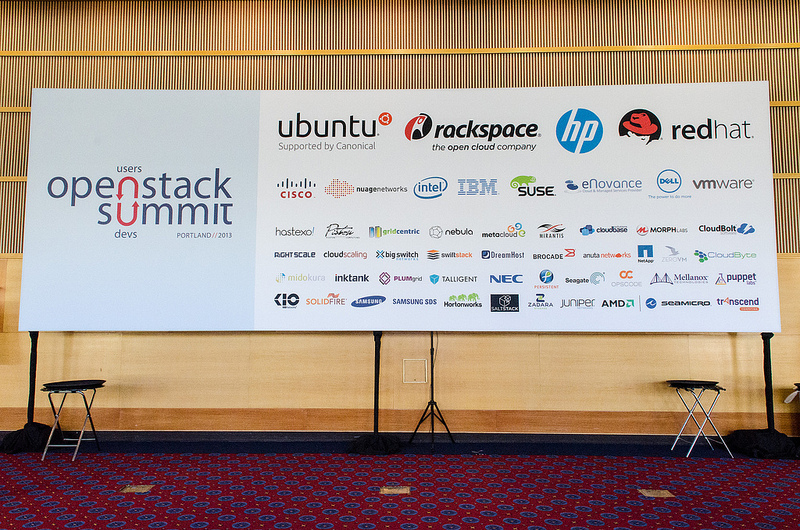
\includegraphics[width=\textwidth]{images/osdevdays.jpg}
\end{center}
\end{frame}



\begin{frame}
\frametitle{OpenStack is People}

% Openstack, rax and NASA in 2010. Ubuntu, then Red Hat, then lots of others

% Components, compatibility

\begin{itemize}
\item 2010: Rackspace (Swift) \& Nasa (Nova)
\item 2011: Ubuntu 11.04 % Deutche Telekom, Carrier Grade OpenStack
\item 2012: Red Hat, Debian (previews)
\item 2013: Red Hat, Debian
\end{itemize}
\end{frame}

\begin{frame}
\begin{center}
     
\includegraphics[width=200pt]{images/bigdeal.jpg}
\end{center}
\end{frame}



\begin{frame}
\begin{center}
\href{http://docs.openstack.org/trunk/install-guide/install/apt/content/figures/1/figures/openstack\_havana\_conceptual\_arch.png}
     {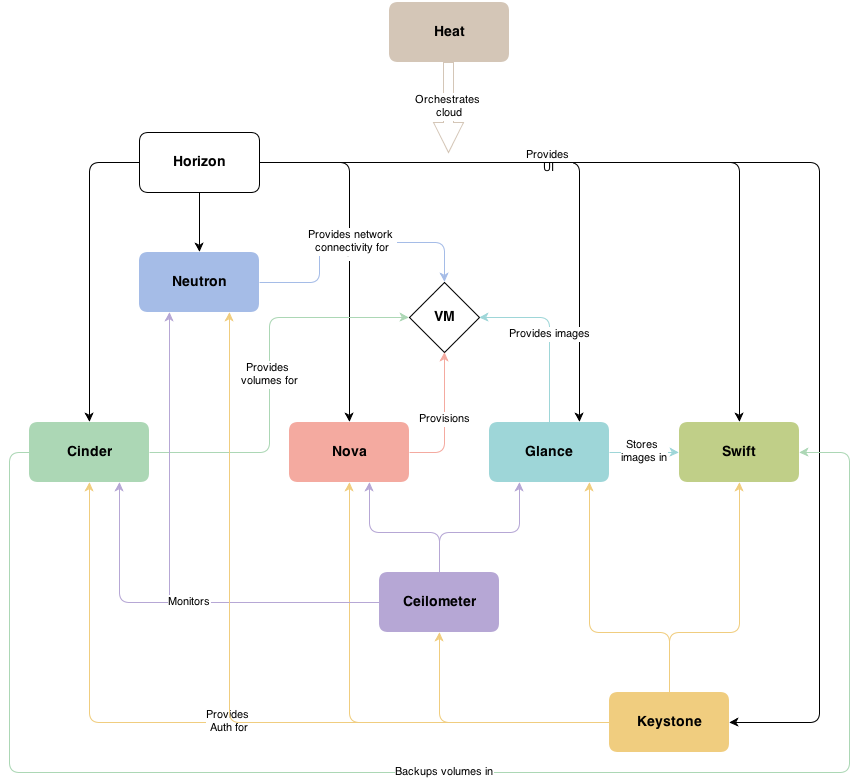
\includegraphics[width=\textwidth]{images/openstack_havana_conceptual_arch.png}}
\end{center}
\end{frame}



\begin{frame}
\begin{center}
\href{http://docs.openstack.org/trunk/install-guide/install/apt/content/figures/2/figures/openstack-arch-havana-logical-v1.jpg}
     {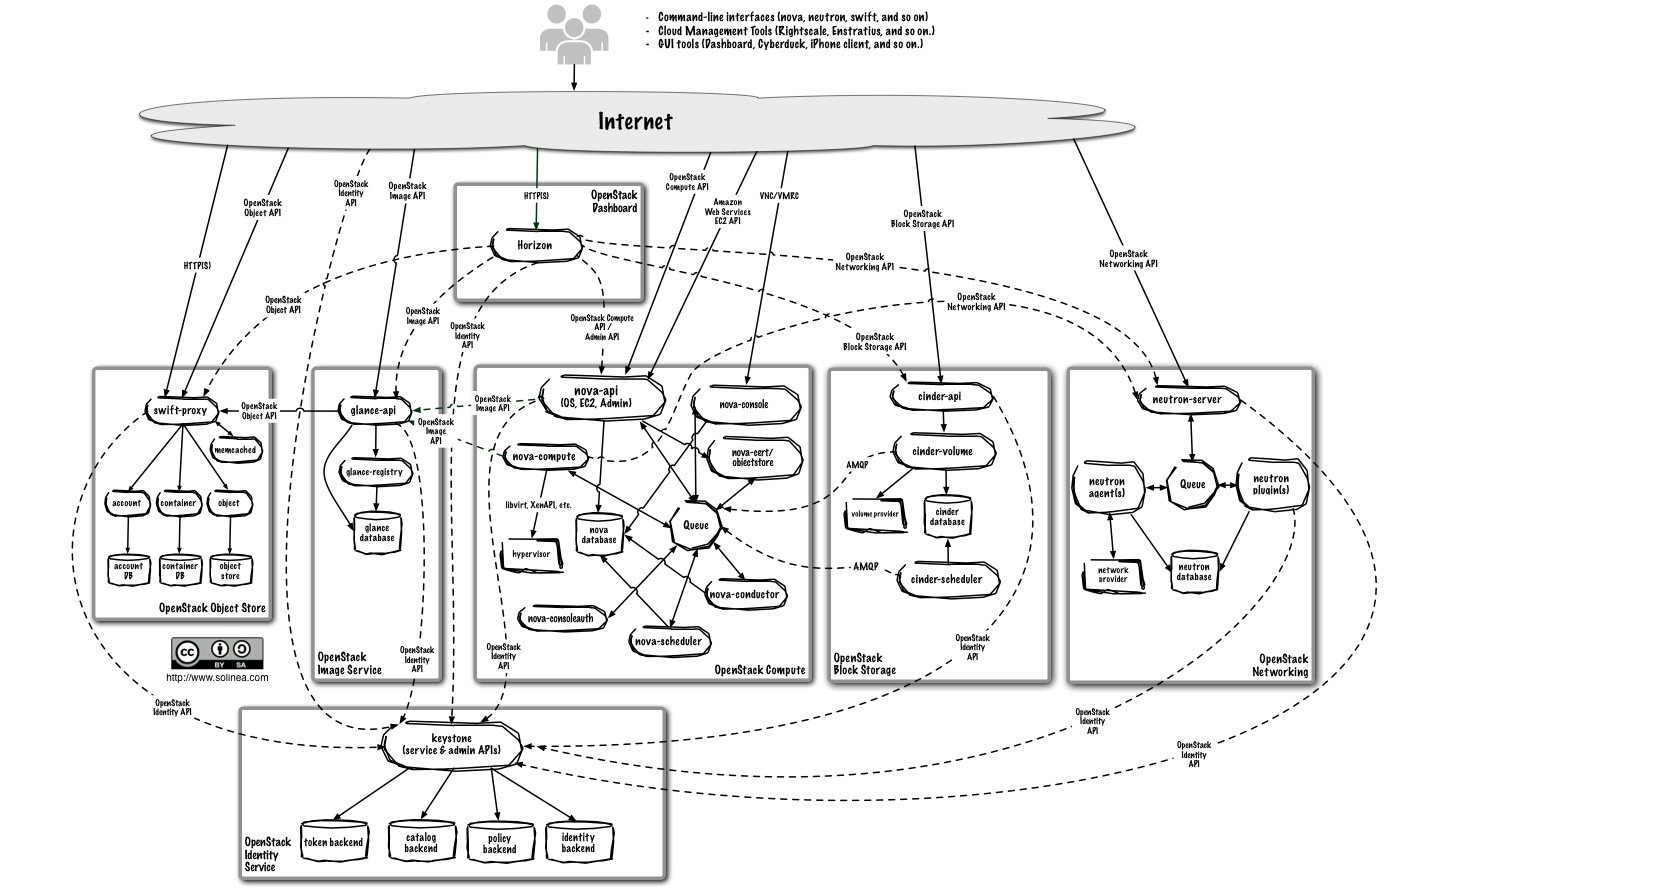
\includegraphics[width=\textwidth]{images/openstack-arch-havana-logical-v1.jpg}}
\end{center}
\end{frame}

\begin{frame}
\frametitle{Nova, Swift, Glance, Grizzly...}

\begin{itemize}
\item \href{http://docs.openstack.org/trunk/install-guide/install/apt/content/ch\_overview.html}{Install Guide for trunk}
\item See components, structure, etc
\end{itemize}

\end{frame}

\begin{frame}
\begin{center}
     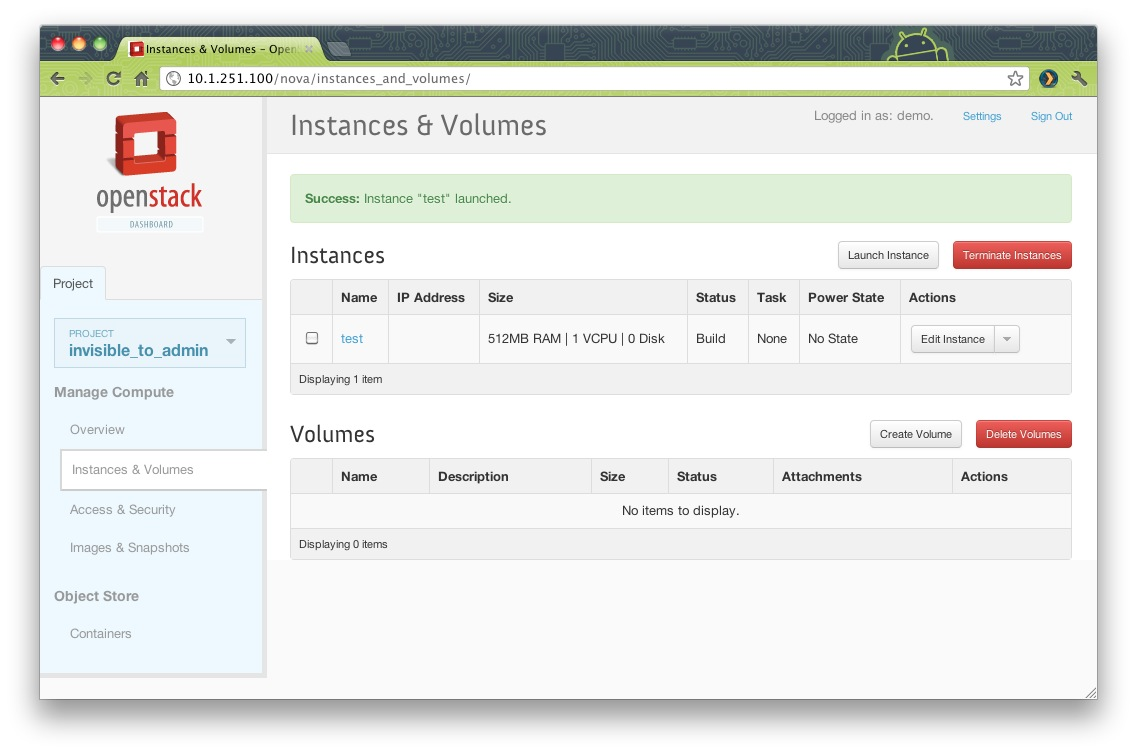
\includegraphics[width=\textwidth]{images/horizon.jpg}
\end{center}
\end{frame}

\begin{frame}
\begin{center}
     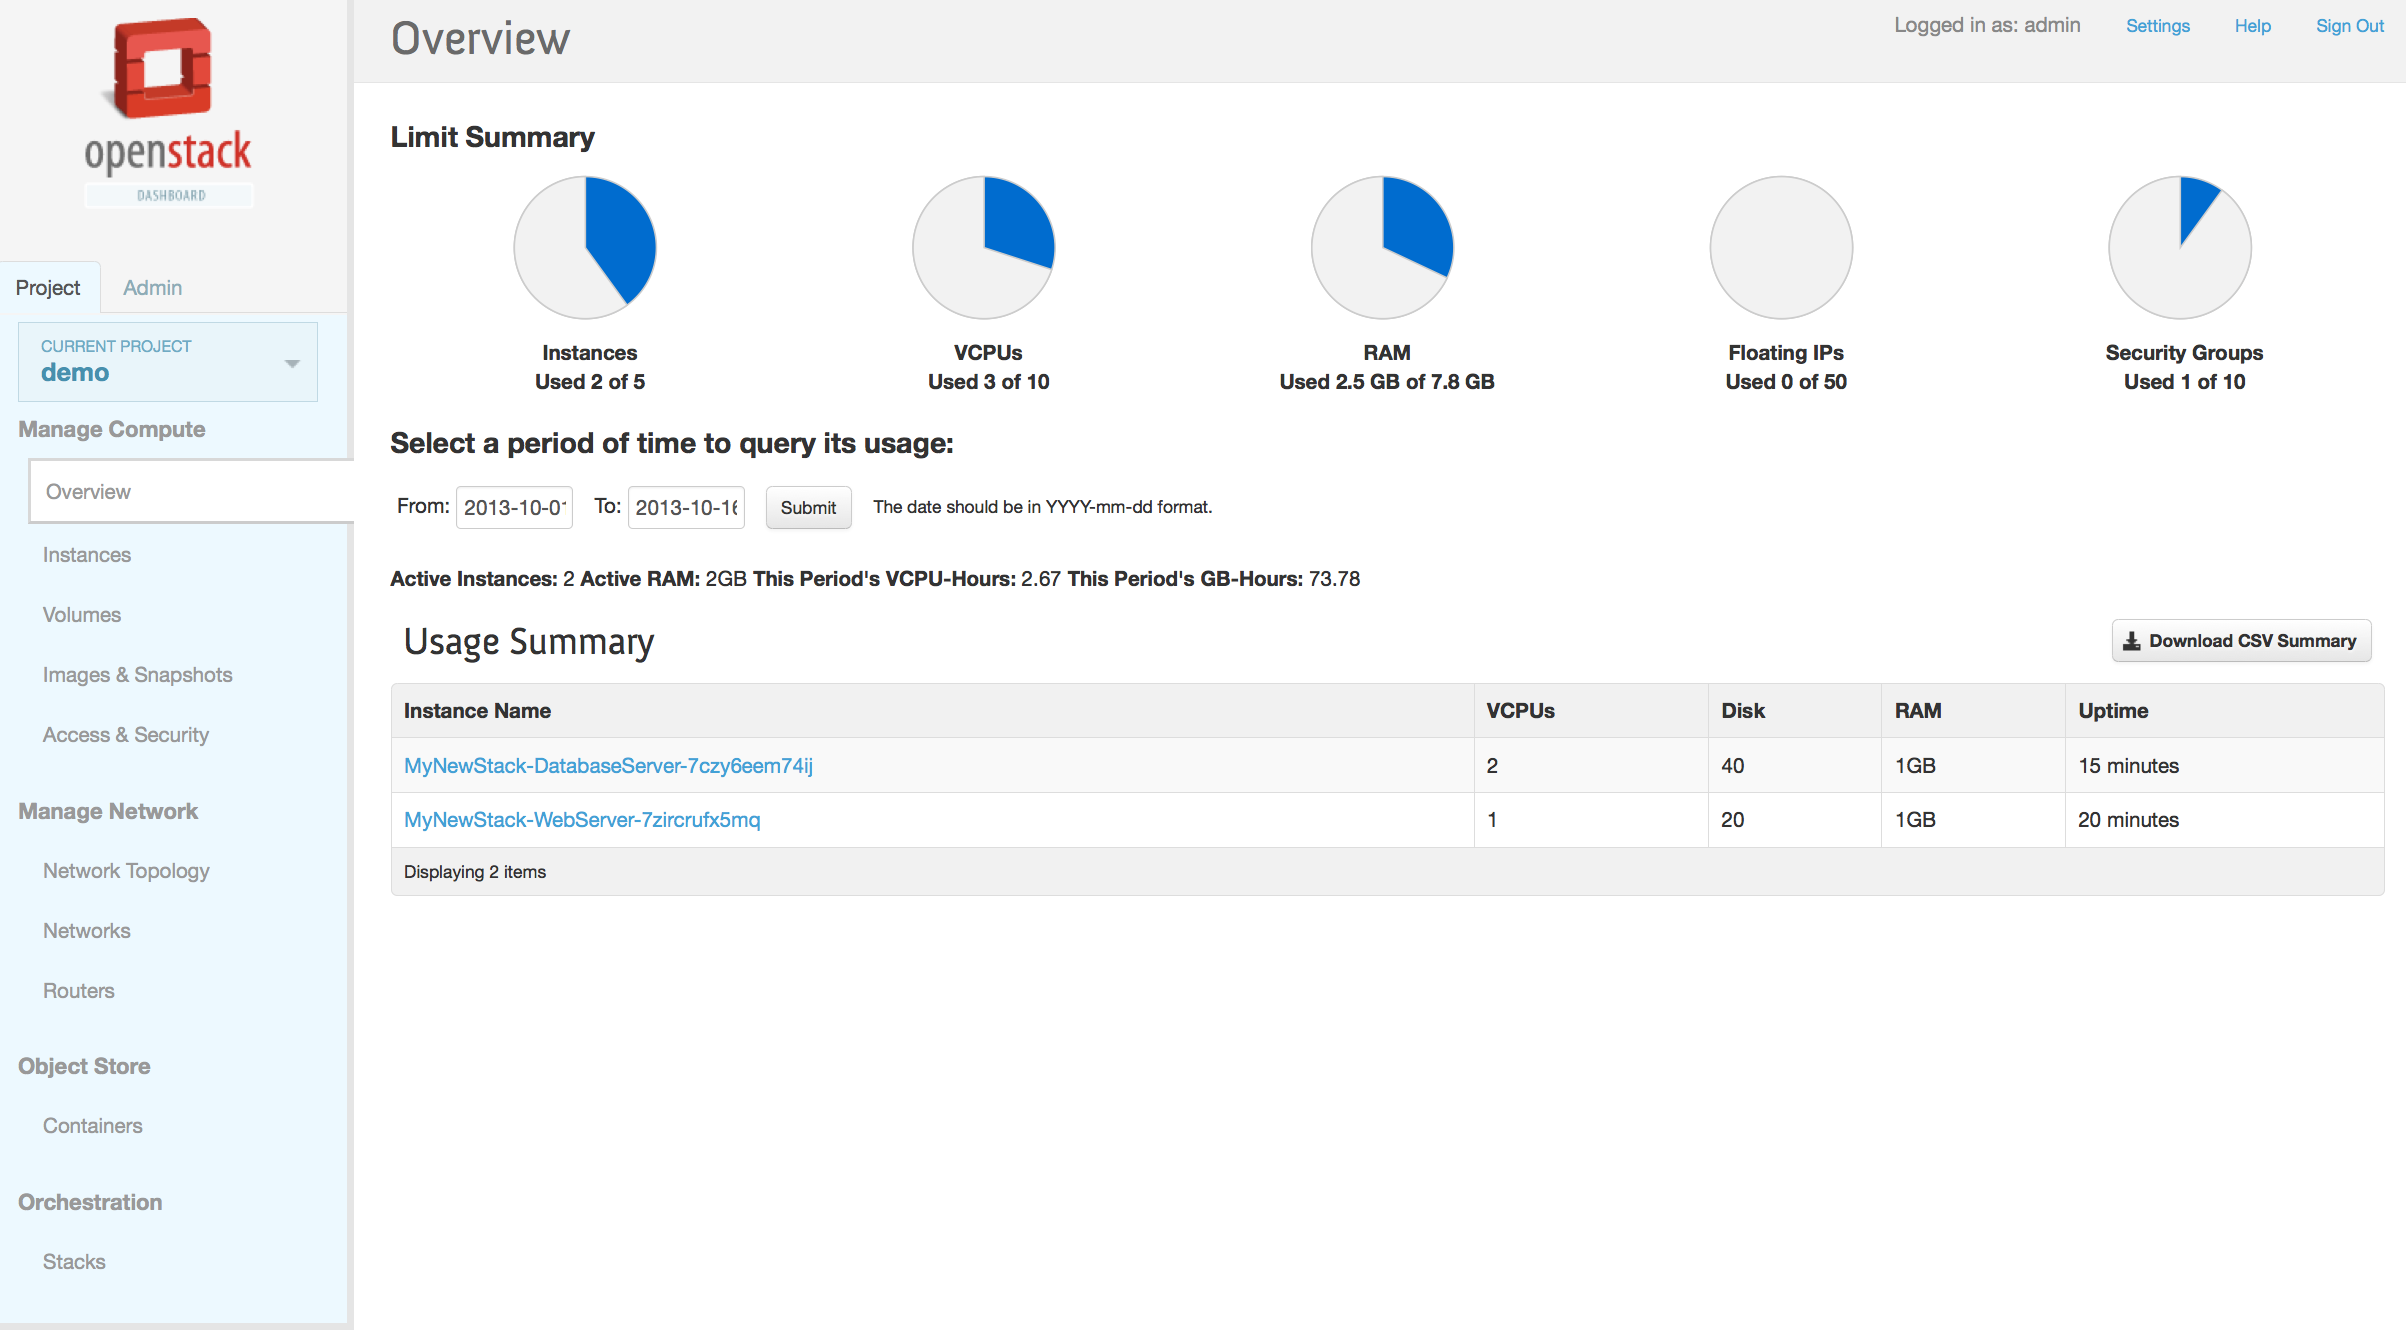
\includegraphics[width=\textwidth]{images/interfaceimprovements.png}
\end{center}
\end{frame}

\begin{frame}
\frametitle{*LIVE* Demo}
% Never do this. \\

\begin{tt}
export OS\_REGION\_NAME="HKG" \\
export OS\_AUTH\_URL=https://id.api.example.com/v2.0/ \\
export OS\_USERNAME=openstack\_username \\
export OS\_PASSWORD=USE\_KEYRING \\
export OS\_TENANT\_NAME=nova-production \\
export OS\_AUTH\_SYSTEM=rackspace \\
export NOVA\_SERVICE\_NAME=cloudServersOpenStack \\
export OS\_PROJECT\_ID=12345 \\
export OS\_NO\_CACHE=1
\end{tt}
\end{frame}

\begin{frame}
\frametitle{*LIVE* Demo (2)}
% Never do this. \\

\begin{tt}

% show some of the flavor-list, image-list, keypair-list, network-list

iad \\
snr boot gatorlug-test --flavor performance1-1 --image 2ab974de-9fe5-4f5b-9d58-766a59f3de61 --key-name cloudhosts --poll \\
snr show gatorlug-test \\
ssh -l root 162.242.244.186 -i ~/.ssh/id\_rsa\_cloudhosts \\
snr delete gatorlug-test \\
\end{tt}
\end{frame}

\begin{frame}
\frametitle{Beyond the examples...}

% Demo nova, swift, talk about APIs that exist - what they provide (auth, retry, paging, polling, edges)

\begin{itemize}

% yum install python-PROJECTclient (swift, nova, neutron, keystone, heat, glance, cinder ceilometer)
\item \href{http://docs.openstack.org/user-guide/content/install\_clients.html}{Command line clients} for everything

% java, python, ruby, php, node, .net
\item \href{http://docs.rackspace.com}{SDKs} for various language environments
\end{itemize}

\end{frame}

\frame{\href{https://github.com/martinb3/DevOps-Challenges-Cycle1}{Examples of the SDKs...}}

\begin{frame}
\frametitle{Get OpenStack}
% DevStack, rax dev accounts (dev trial)

Complete Environment - \href{http://devstack.org/}{devstack.org}

Rackspace Loves Developers - \href{http://developer.rackspace.com/devtrial/}{developer.rackspace.com/devtrial}
 
% When you sign up today, you will get USD $300 in free cloud services - that's up to USD $50 per month credit for six months on your Rackspace Cloud account, powered by OpenStack™.

% The discount does apply to new products, such as our Performance Cloud Servers, Cloud Queues, and other products we launch. Additionally, you are eligible for early access to new features and products we may roll out. 

\end{frame}

\begin{frame}
% OpenStack Ironic (Baremetal)
Infrastructure as an API -- \href{https://wiki.openstack.org/wiki/Baremetal}{Project Ironic} \\
Developer Portal -- \href{http://developer.rackspace.com}{developer.rackspace.com}


% Proof that OpenStack is NOT the same thing as VMware, VirtualBox
% "Baremetal cloud"

\end{frame}

\begin{frame}
\begin{center}
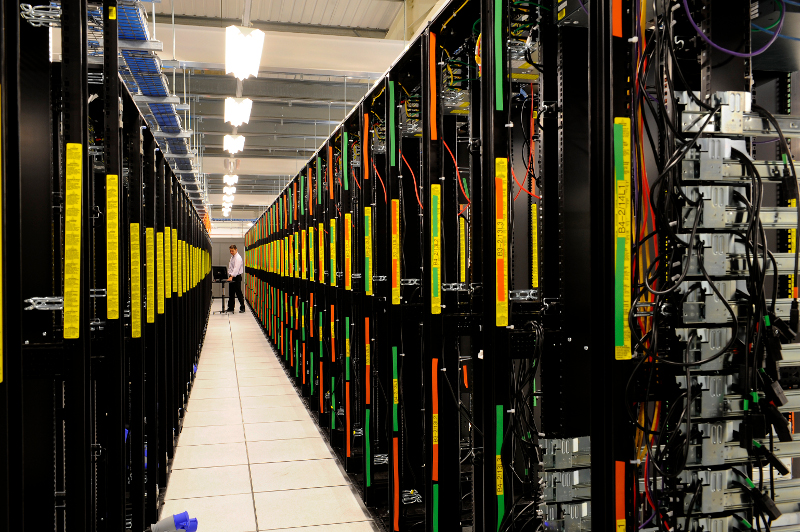
\includegraphics[width=\textwidth]{images/raxdc.jpg}
\end{center}
\end{frame}

\frame{Questions? Answers!}

\end{document}



